\documentclass{standalone}
\usepackage[ascii]{inputenc}
\usepackage{tikz}

\tikzstyle{arrow} = [draw, thick, -stealth]

\begin{document}

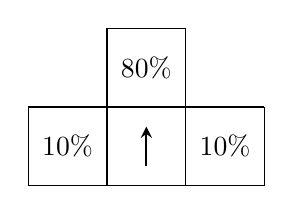
\begin{tikzpicture}
\draw (-1,0) -- ( 2,0);
\draw (-1,1) -- ( 2,1);
\draw ( 0,0) -- ( 0,2);
\draw ( 1,0) -- ( 1,2);
\draw ( 0,2) -- ( 1,2);
\draw (-1,0) -- (-1,1);
\draw ( 2,0) -- ( 2,1);
\draw [arrow] (0.5,0.25) -- (0.5,0.75);
\node at ( 0.5,1.5) {$80\%$};
\node at (-0.5,0.5) {$10\%$};
\node at ( 1.5,0.5) {$10\%$};
\end{tikzpicture}

\end{document}
